\documentclass{article}




\usepackage{fullpage}
\usepackage{nopageno}
\usepackage{amsmath}
\usepackage{amsfonts}
\usepackage{graphicx}
\usepackage{framed}
\usepackage{xcolor}

\definecolor{dark_red}{rgb}{0.5,0.0,0.0}
\definecolor{dark_green}{rgb}{0.0,0.5,0.0}
\definecolor{dark_blue}{rgb}{0.0,0.0,0.5}
\definecolor{blue}{rgb}{0.0,0.0,1.0}

\newcommand{\dr}[1]{\textcolor{dark_red}{#1}}
\newcommand{\dg}[1]{\textcolor{dark_green}{#1}}
\newcommand{\db}[1]{\textcolor{dark_blue}{#1}}
\newcommand{\blue}[1]{\textcolor{blue}{#1}}




\begin{document}

\section*{About division}

To ``divide" a number \(a\) by another number \(b\), is to either split \(a\) into \(b\) equal parts, or to count the number of copies of \(b\) required to sum to \(a\). There are two views of division, that give the exact same result:

\begin{description}
\item[Partition Division] After splitting \(a\) into \(b\) equal parts, the quotient \(a/b\) is the size of a single part. 
\item[Quotition Division] The quotient \(a/b\) is the number of copies of \(b\) that need to be summed to get a total of \(a\).
\end{description}

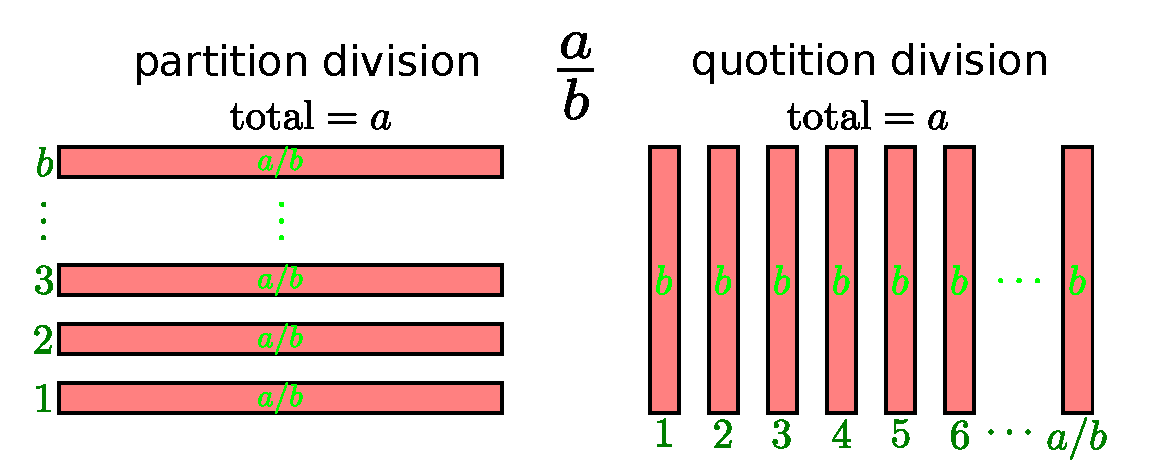
\includegraphics[width = \textwidth]{two_approaches_to_division}

It is important to note that no matter which view of division is being used, the result is always the same. Below is given a series of example quotients where the partition and quotition interpretations of division are presented side by side. It should be noted that the interpretation, partition or quotition, has no effect on the value of the quotient. Why is the distinction important? The distinction helps in deciding when to use division, and it also helps in the understanding of the algebraic rules surrounding division. 

When it comes to {\bf computing} the quotients, the quotition interpretation is the interpretation that is almost always used. The quotient \(a/b\) is computed by counting the number of copies of \(b\) that can be taken from \(a\). Despite this, the partition interpretation still sees use in identifying scenarios where division is to be used, establishes the notion of fractions, is the literal interpretation of the word ``division", and is the first interpretation of division that is taught to students.

\vspace{5mm}

%%%%%%%%%%%%%%%%%%%%%%%%%%%%

In the image below, the quotient \(\frac{6}{2} = 3\) is depicted via both partition and quotition. 
\begin{itemize}
\item On the left, partitioning is used to split \(6\) into \(2\) equal parts. The size of a single part is \(3\). 
\item On the right, quotitioning is used. \(3\) is the number of copies of \(2\) that need to be summed to total \(6\). 
\end{itemize}
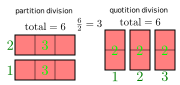
\includegraphics[width = \textwidth]{6_div_2}

\vspace{5mm}

%%%%%%%%%%%%%%%%%%%%%%%%%%%%

In the image below, the quotient \(\frac{12}{3} = 4\) is depicted via both partition and quotition. 
\begin{itemize}
\item On the left, partitioning is used to split \(12\) into \(3\) equal parts. The size of a single part is \(4\). 
\item On the right, quotitioning is used. \(4\) is the number of copies of \(3\) that need to be summed to total \(12\). 
\end{itemize}
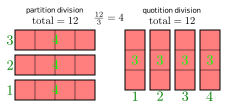
\includegraphics[width = \textwidth]{12_div_3}

\vspace{5mm}

%%%%%%%%%%%%%%%%%%%%%%%%%%%%

In the image below, the quotient \(\frac{7}{2} = 3.5\) is depicted via both partition and quotition. 
\begin{itemize}
\item On the left, partitioning is used to split \(7\) into \(2\) equal parts. The size of a single part is \(3.5\). 
\item On the right, quotitioning is used. \(3.5\) is the number of copies of \(2\) that need to be summed to total \(7\). With the quotitioning, note that a \(0.5\) copy of \(2\) is need to finish the total. 
\end{itemize}
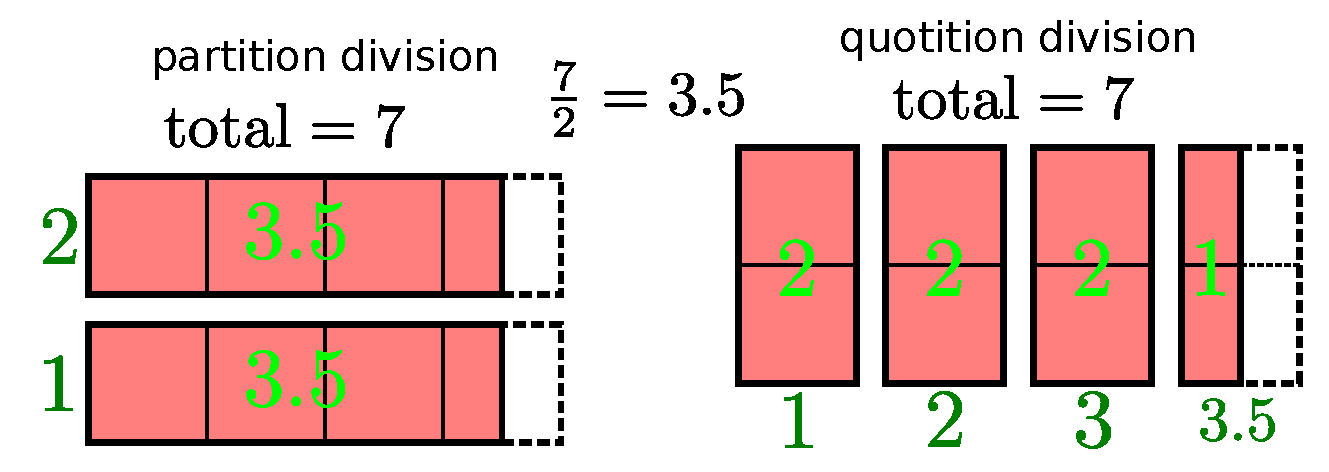
\includegraphics[width = \textwidth]{7_div_2}

\vspace{5mm}

%%%%%%%%%%%%%%%%%%%%%%%%%%%%

\begin{tabular}{cc}
\parbox{0.5\textwidth}{
In the image to the right, the quotient \(\frac{7}{3.5} = 2\) is depicted via both partition and quotition. 
\begin{itemize}
\item On the left, partitioning is used to split \(7\) units into \(3.5\) equal parts. Note that \(0.5\) of a part is \(50\%\) the size of a whole part. The quotient is the size of a full part which is \(2\) units. 
\item On the right, quotitioning is used. \(2\) is the number of copies of \(3.5\) that need to be summed to total \(7\). 
\end{itemize}
} & \parbox{0.5\textwidth}{
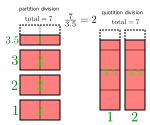
\includegraphics[width = 0.5\textwidth]{7_div_3p5}
}
\end{tabular}

\vspace{5mm}

%%%%%%%%%%%%%%%%%%%%%%%%%%%%

In the image below, the quotient \(\frac{8.75}{2.5} = 3.5\) is depicted via both partition and quotition. 
\begin{itemize}
\item On the left, partitioning is used to split \(8.75\) units into \(2.5\) equal parts. Note that \(0.5\) of a part is \(50\%\) the size of a whole part. The quotient is the size of a full part which is \(3.5\) units. 
\item On the right, quotitioning is used. \(3.5\) is the number of copies of \(2.5\) that need to be summed to total \(7\). With the quotitioning, note that a \(0.5\) copy of \(2.5\) is need to finish the total. 
\end{itemize}
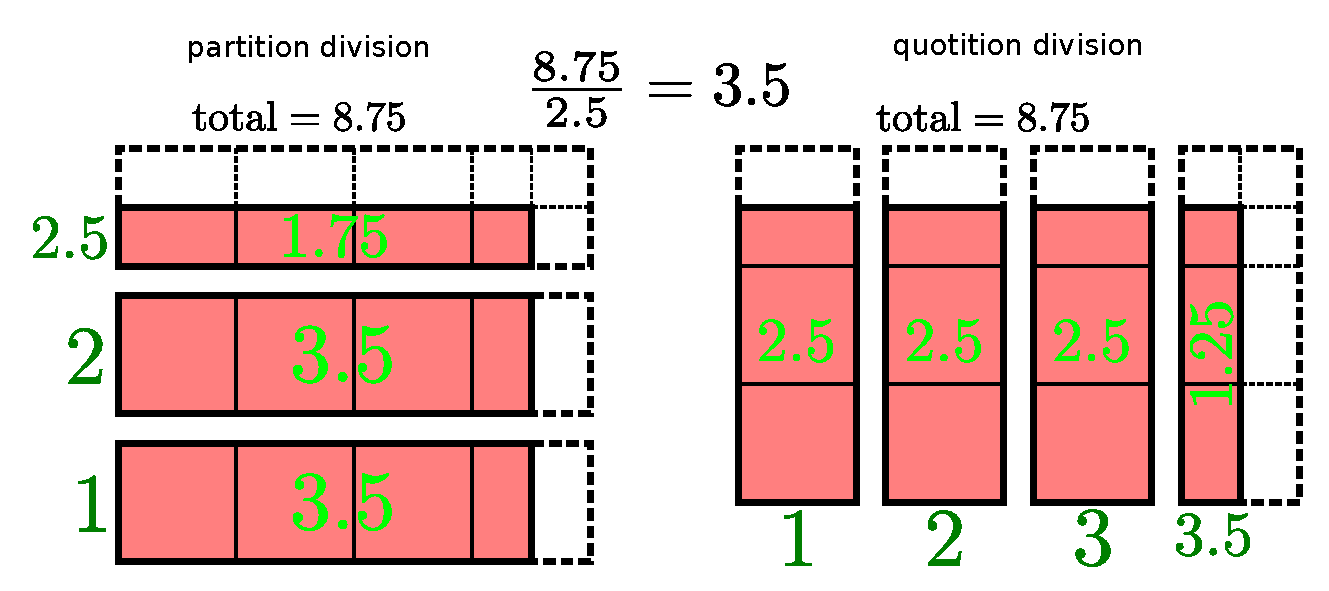
\includegraphics[width = 0.8\textwidth]{8p75_div_2p5}

\vspace{5mm}

%%%%%%%%%%%%%%%%%%%%%%%%%%%%

\begin{tabular}{cc}
\parbox{0.5\textwidth}{
In the image to the right, the quotient \(\frac{1}{3}\) is depicted via both partition and quotition. 
\begin{itemize}
\item On the left, partitioning is used to split \(1\) into \(3\) equal parts. 
\item On the right, quotitioning is used. \(1/3\) of a copy of \(3\) is needed to total to \(1\). 
\end{itemize}
} & \parbox{0.5\textwidth}{
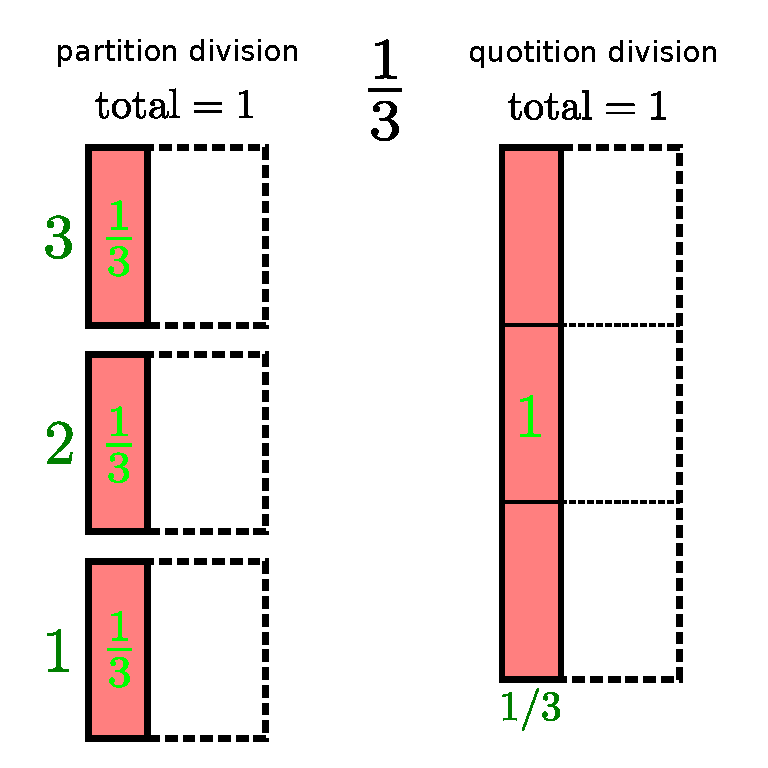
\includegraphics[width = 0.5\textwidth]{1_div_3}
}
\end{tabular}

\vspace{5mm}

%%%%%%%%%%%%%%%%%%%%%%%%%%%%

\begin{tabular}{cc}
\parbox{0.4\textwidth}{
In the image to the right, the quotient \(\frac{1.8}{4.5} = 0.4\) is depicted via both partition and quotition. 
\begin{itemize}
\item On the left, partitioning is used to split \(1.8\) units into \(4.5\) equal parts. Note that \(0.5\) of a part is \(50\%\) the size of a whole part. The quotient is the size of a full part which is \(0.4\) units.
\item On the right, quotitioning is used. \(0.4\) of a copy of \(4.5\) is needed to total to \(1.8\). 
\end{itemize}
}
& \parbox{0.5\textwidth}{
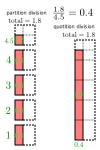
\includegraphics[width = 0.5\textwidth]{1p8_div_4p5}
}
\end{tabular}

\vspace{5mm}

%%%%%%%%%%%%%%%%%%%%%%%%%%%%

When \(b\) becomes less then \(1\), splitting \(a\) into \(b\) equal parts becomes less intuitive. Below, the quotient \(\frac{1.5}{0.5} = 3\) is depicted via both partition and quotition. 
\begin{itemize}
\item On the left, partitioning is used to split \(1.5\) units into \(0.5\) equal parts. Normally the numerator of \(a = 1.5\) units is split between multiple parts. Here instead, the \(0.5\) part receives all of the \(a = 1.5\) units. The quotient is the size of a whole part however, and a whole part is \(2\) times the size of a \(0.5\) part. The size of a ``whole part" is therefore \(2 \times 1.5 = 3\) units. 
\item On the right, quotitioning is used. \(3\) is the number of copies of \(0.5\) is needed to total to \(1.5\).  
\end{itemize}
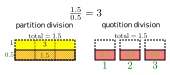
\includegraphics[width = 0.8\textwidth]{1p5_div_0p5}

\vspace{5mm}

%%%%%%%%%%%%%%%%%%%%%%%%%%%%

Below, the quotient \(\frac{1.8}{0.4} = 4.5\) is depicted via both partition and quotition. 
\begin{itemize}
\item On the left, partitioning is used to split \(1.8\) units into \(0.4\) equal parts. Normally the numerator \(a = 1.8\) units is split between multiple parts. Here instead, the \(0.4\) part receives all of \(a = 1.8\) units. The quotient is the size of a whole part however, and a whole part is multiple copies of a \(0.4\) part (\(2.5\) copies to be exact). The size of a ``whole part" is \(4.5\) units. 
\item On the right, quotitioning is used. \(4.5\) is the number of copies of \(0.4\) is needed to total to \(1.8\). Note that a \(0.5\) copy of \(0.4\) is needed to finish the total.  
\end{itemize}
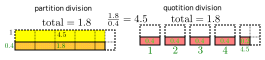
\includegraphics[width = \textwidth]{1p8_div_0p4}

\vspace{5mm}

%%%%%%%%%%%%%%%%%%%%%%%%%%%%

Below, the quotient \(\frac{-5}{2} = -2.5\) is depicted via both partition and quotition. 
\begin{itemize}
\item On the left, partitioning is used to split \(-5\) into \(2\) equal parts. The size of a single part is \(-2.5\). 
\item On the right, quotitioning is used. \(2.5\) negative copies of \(2\) are required to form the total of \(a = -5\) units. Each negative copy subtracts \(1\) from the total number of copies, so the number of copies is \(-2.5\). Note that a \(-0.5\) copy of \(2\) is needed to finish the total. 
\end{itemize}
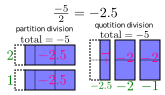
\includegraphics[width = 0.8\textwidth]{m5_div_2}

\vspace{5mm}

%%%%%%%%%%%%%%%%%%%%%%%%%%%%

Below, the quotient \(\frac{5}{-2} = -2.5\) is depicted via both partition and quotition. 
\begin{itemize}
\item On the left, partitioning is used to split \(5\) into \(-2\) equal parts. This is done by splitting the \(a = 5\) units evenly between \(2\) parts that each have a negative weight of \(-1\). Each negative part gets \(2.5\) units. The quotient however is the number of units that would be in a positive whole part. A positive whole part has a weight of \(+1\). A part with a weight of \(-1\) is getting \(2.5\) units, so a part with a weight of \(+1\) would get \(-2.5\) units, hence the quotient is \(-2.5\).
\item On the right, quotitioning is used. \(2.5\) negative copies of \(-2\) are required to form the total of \(a = 5\) units. Each negative copy subtracts \(1\) from the total number of copies, so the number of copies is \(-2.5\). Note that a \(-0.5\) copy of \(-2\) is needed to finish the total. 
\end{itemize}
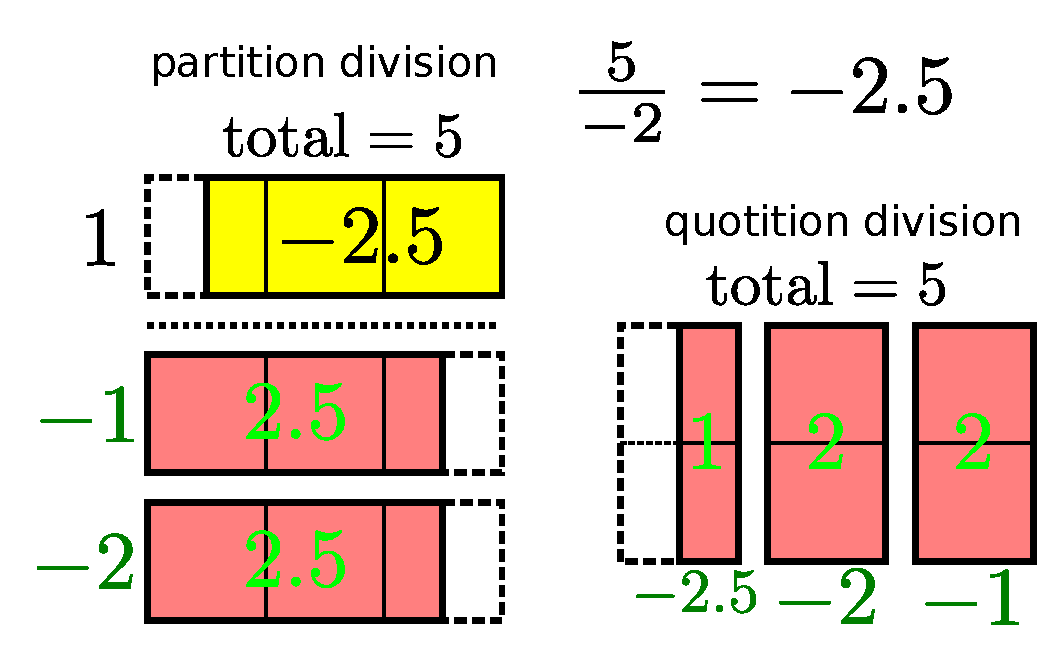
\includegraphics[width = 0.8\textwidth]{5_div_m2}

\vspace{5mm}

%%%%%%%%%%%%%%%%%%%%%%%%%%%%

Below, the quotient \(\frac{-5}{-2} = 2.5\) is depicted via both partition and quotition. 
\begin{itemize}
\item On the left, partitioning is used to split \(-5\) into \(-2\) equal parts. This is done by splitting the \(a = -5\) units evenly between \(2\) parts that each have a negative weight of \(-1\). Each negative part gets \(-2.5\) units. The quotient however is the number of units that would be in a positive whole part. A positive whole part has a weight of \(+1\). A part with a weight of \(-1\) is getting \(-2.5\) units, so a part with a weight of \(+1\) would get \(2.5\) units, hence the quotient is \(2.5\).
\item On the right, quotitioning is used. \(2.5\) copies of \(-2\) are required to form the total of \(a = -5\) units. Note that a \(0.5\) copy of \(-2\) is needed to finish the total. 
\end{itemize}
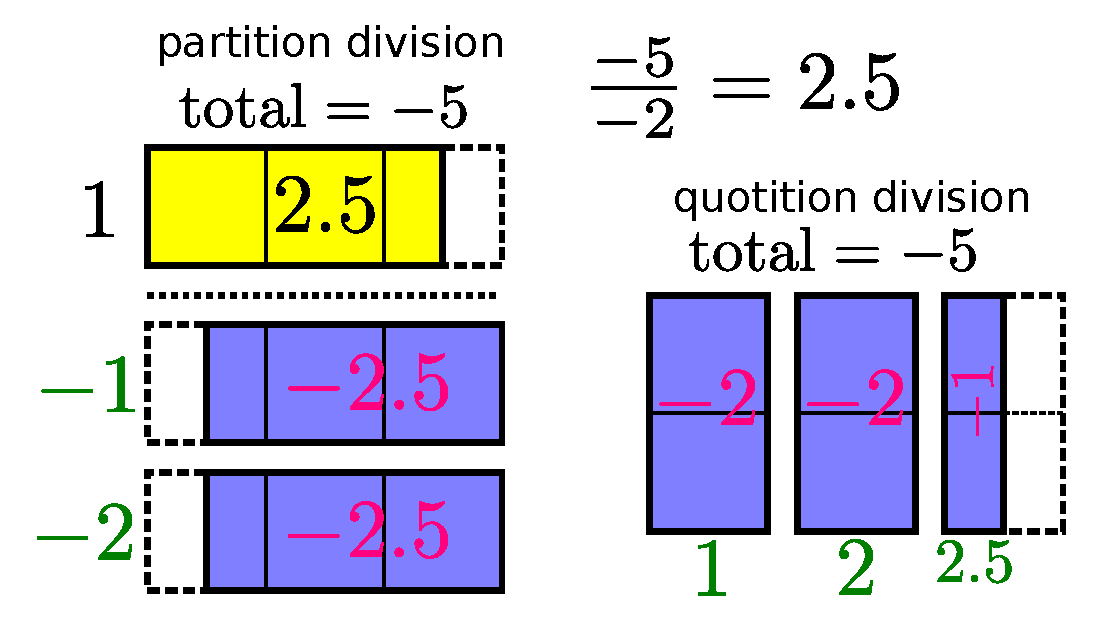
\includegraphics[width = 0.8\textwidth]{m5_div_m2}

\vspace{5mm}

In summary, 
\begin{itemize}
\item With partition division, the quotient \(a/b\) is the value of a {\bf whole part} after \(a\) has been split into \(b\) equal parts. When \(b\) is not a positive integer, the following must clarified: 
\begin{itemize}
\item[*] When \(b\) has a fractional part, the value of the fractional part is the corresponding proportion of a full part. For instance, a \(0.5\) part has \(1/2\) the value of a full part, and a \(0.1\) part has \(1/10\) the value of a full part. \(a/b\) is the value of a full part, and not of any fractional part. 
\item[*] When \(b\) is negative, the value of a negative part is the negative of the value of a full part. If a negative part has a value of \(3\), then a full part has a value of  \(-3\). \(a/b\) is the value of a full part, and not of any negative part. 
\end{itemize}
\item With quotition division, the quotient \(a/b\) is the {\bf number of copies} of \(b\) that need to be summed to get \(a\). When \(a/b\) is not a positive integer, the following must clarified: 
\begin{itemize}
\item[*] When \(a/b\) has a fractional part, the contents of the fractional copy of \(b\) has the corresponding proportion of a full copy of \(b\). For instance, a \(0.5\) copy of \(b\) has \(1/2\) the value of \(b\), and a \(0.1\) copy has \(1/10\) the value of \(b\).
\item[*] When \(a/b\) is negative, the value of a negative copy of \(b\) is \(-b\).
\end{itemize}
\end{itemize}





\section*{Division identities}

The various algebraic rules (identities) concerning division can be understood using a mixture of the partition interpretation and the quotition interpretation of division.

%%%%%%%%%%%%%%%%%%%%%%%%%%%%

Given any real numbers \(a\), \(b\), and \(c\), the division of the product \(ab\) by \(c\) is equivalent to the product \(a \cdot \frac{b}{c}\):
\[\frac{ab}{c} = a \cdot \frac{b}{c}\]
This equation can be understood in the following ways:
\begin{itemize}
\item \textbf{Partition division:} The product \(ab\) is \(a\) copies of \(b\). \(\frac{ab}{c}\) is the product \(ab\) split into \(c\) equal pieces. Splitting \(ab\) into \(c\) equal pieces can be done by splitting each of the \(a\) copies of \(b\) into \(c\) equal pieces to get \(a\) copies of \(\frac{b}{c}\). This understanding is depicted in the image below on the left where an area of \(ab\) is split into \(c\) equal columns, and each column is \(a\) copies of \(\frac{b}{c}\). 
\item \textbf{Quotition division:} \(\frac{ab}{c}\) is the number of copies of \(c\) that need to be summed to get \(ab\). \(\frac{b}{c}\) is the number of copies of \(c\) that need to be summed to get \(b\). \(a\) copies of \(\frac{b}{c}\) is a number of copies of \(c\) that when summed gives \(a\) copies of \(b\) which is \(ab\). This understanding is depicted in the image below on the right where \(a \cdot \frac{b}{c}\) copies of \(c\) sum to \(ab\). 
\end{itemize}
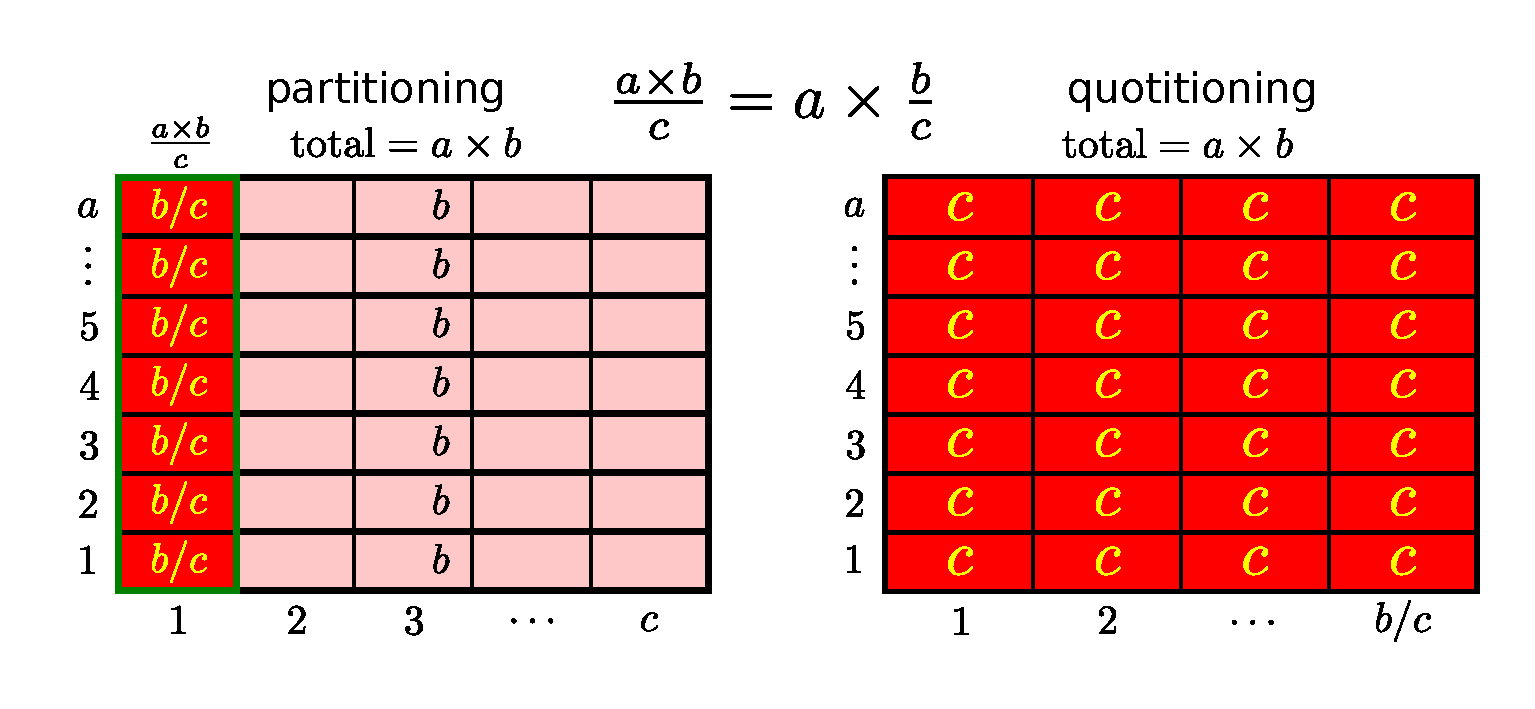
\includegraphics[width = \textwidth]{ab_div_c_equals_a_times_b_div_c}

For example, the expression \(\frac{a}{b}\) is taught in elementary school to mean \(a\) copies of \(\frac{1}{b}\). The above identity makes it clear that \(\frac{a}{b}\) is also \(a\) divided into \(b\) equal parts. This is why the fraction bar ``\(/\)" replaces the division symbol \(\div\).

\vspace{5mm}

%%%%%%%%%%%%%%%%%%%%%%%%%%%%

\begin{tabular}{cc}
\parbox{0.5\textwidth}{
Given any real numbers \(a\), \(b\), and \(c\), dividing \(a\) by \(b\), and then dividing by \(c\) is equivalent to a straightforwards division of \(a\) by the product \(bc\):
\[\frac{a/b}{c} = \frac{a}{bc}\]
This equation is easiest to understand using {\bf partition} division: \\
\(\frac{a}{b}\) is \(a\) divided into \(b\) equal pieces. \(\frac{a/b}{c}\) is a further division of \(\frac{a}{b}\) into \(c\) equal pieces. \(c\) copies of \(\frac{a/b}{c}\) is \(\frac{b}{a}\). \(b\) copies of \(c\) copies of \(\frac{a/b}{c}\) is \(b\) copies of \(\frac{a}{b}\) which in turn is \(a\). Therefore \(bc\) copies of \(\frac{a/b}{c}\) is \(a\). \(\frac{a/b}{c}\) is \(a\) divided into \(bc\) equal pieces.
} & \parbox{0.5\textwidth}{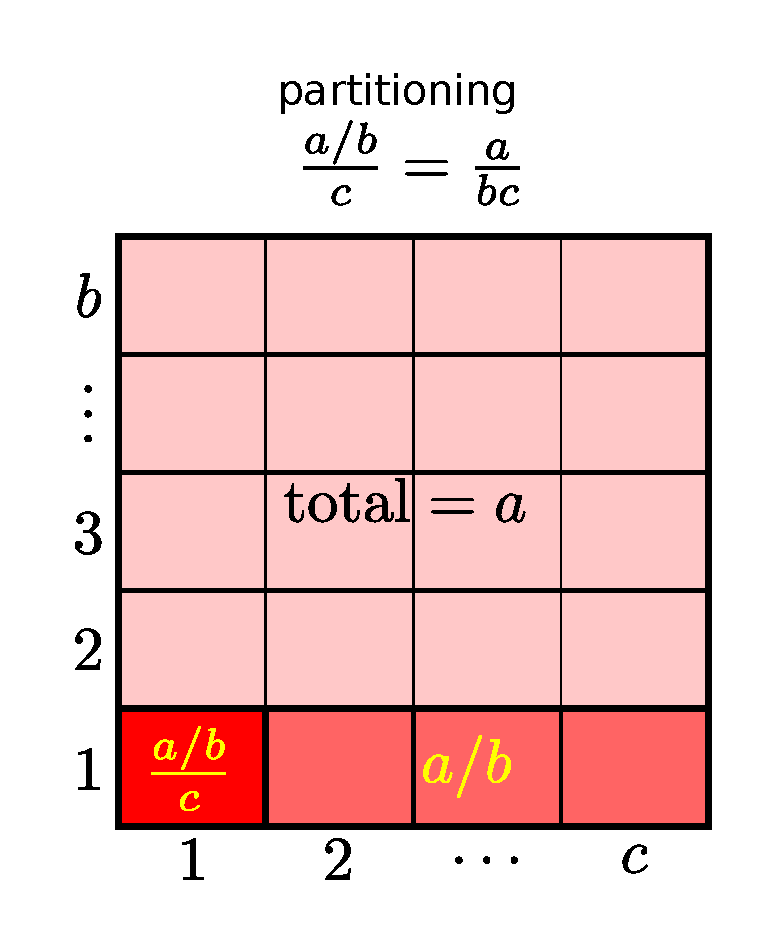
\includegraphics[width = 0.5\textwidth]{a_div_b_div_c_equals_a_div_bc}}
\end{tabular}

\vspace{5mm}

%%%%%%%%%%%%%%%%%%%%%%%%%%%%

Given any real numbers \(a\) and \(b\), the division of \(a\) by \(1/b\) is the product \(ab\):
\[\frac{a}{1/b} = ab\]
The division of \(a\) into ``\(\frac{1}{b}\)" equal parts can be difficult to grasp, so the {\bf quotition} interpretation of division will used instead. \(b\) copies of \(\frac{1}{b}\) sum to \(1\) since \(\frac{1}{b}\) is \(1\) split into \(b\) equal pieces. \(ab\) copies of \(\frac{1}{b}\) sum to \(a\) copies of \(1\) which is \(a\). The product \(ab\) is the number of copies of \(\frac{1}{b}\) that need to be summed to get \(a\). This is illustrated in the image below. \\
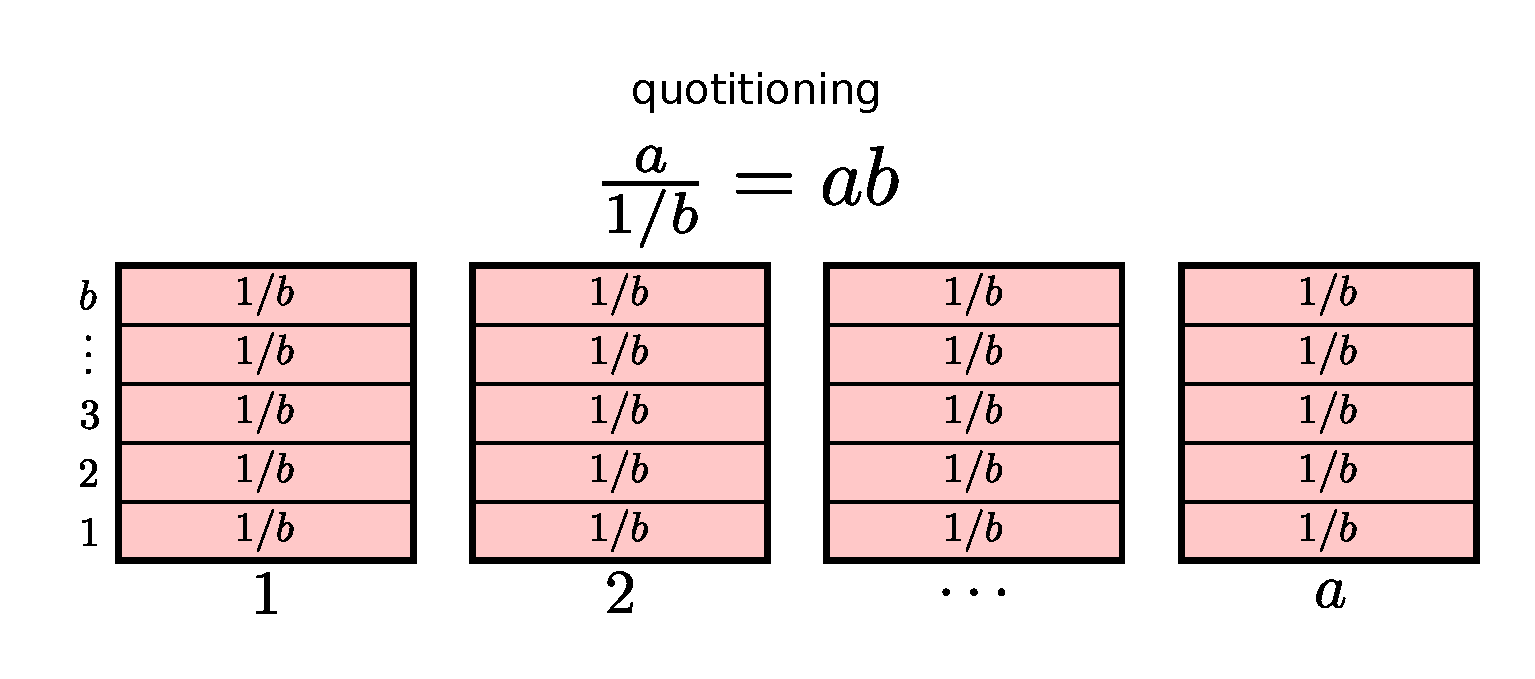
\includegraphics[width = \textwidth]{a_div_(1_div_b)_equals_ab}





\section*{About ratios}

When two quantities \(Q_1\) and \(Q_2\) (concrete examples will be given later) are ``proportional" to each other, there are numbers \(a\) and \(b\) such that any collection of \(a\) units of quantity \(Q_1\) ``corresponds" to \(b\) units of quantity \(Q_2\). The {\bf ratio} of quantity \(Q_1\) to quantity \(Q_2\) is represented by:
\[a : b\]
Given any real number \(k\), \(k\) copies of \(a\) units of \(Q_1\), \(ka\), ``corresponds" to \(k\) copies of \(b\) units of \(Q_2\), \(kb\), so the ratio \(a : b\) is unchanged if both \(a\) and \(b\) are multiplied by the common multiplier of \(k\):
\[ka : kb = a : b\]

As an example, consider a mystery metal where a volume of \(2.5\text{L}\) has a mass of \(10\text{kg}\). The first quantity \(Q_1\) is ``volume", and the second quantity \(Q_2\) is ``mass". The volume-mass ratio is denoted by 
\[2.5\text{L} : 10\text{kg}\]
\(3\) copies of \(2.5\text{L}\) of the mystery metal has a mass equivalent to \(3\) copies of \(10\text{kg}\). The ratio can also be expressed as:
\[3 \times 2.5\text{L} : 3 \times 10\text{kg} = 7.5\text{L} : 30\text{kg}\]

A very common problem involving ratios is the following:

{\bf If \(a\) units of quantity \(Q_1\) correspond to \(b\) units of quantity \(Q_2\), then \(c\) units of \(Q_1\) correspond to how many units of \(Q_2\)?}

There are two approaches to solving this problem: the ``partition approach" and the ``quotition approach".

{\bf The partition approach}

The partition approach involves first computing the number of units of \(Q_2\) that correspond to a single unit of \(Q_1\). The number of units of \(Q_2\) that correspond to \(1\) unit of \(Q_1\) is determined by distributing the \(b\) units of \(Q_2\) evenly amongst the \(a\) units of \(Q_1\). This is to invoke the partition interpretation of division and split \(b\) into \(a\) equal parts, a single part corresponding to a single unit of \(Q_1\). With \(1\) unit of \(Q_1\) corresponding to \(b/a\) units of \(Q_2\), \(c\) units of \(Q_1\) corresponds to \(c(b/a)\) units of \(Q_2\).

{\bf The quotition approach}

The quotition approach involves first invoking the quotition interpretation of division and compute the number of copies of \(a\) units of \(Q_1\) needed to build up \(c\) units of \(Q_1\). Once \(c/a\) has been computed, each block of \(a\) units of \(Q_1\) is converted to \(b\) units of \(Q_2\). \(c/a\) blocks of \(a\) units of \(Q_1\) becomes \(c/a\) blocks of \(b\) units of \(Q_2\). \(c/a\) blocks of \(b\) units of \(Q_2\) is \((c/a)b\) units of \(Q_2\). 

Both approaches yield the final expression of \(bc/a\).

{\bf Example 1:}

Consider the previous example. A mystery metal where a volume of \(2.5\text{L}\) has a mass of \(10\text{kg}\). In this context, \(Q_1\) is volume, and \(Q_2\) is mass. Two questions will be asked:
\begin{description}
\item[Question 1:] What is the mass of \(75\text{L}\) of this mystery metal?
	\begin{description}
	\item[Partition approach:] The mass per \(1\text{L}\) of metal is: \(\frac{10\text{kg}}{2.5\text{L}} = 4\text{kg/L}\). This is also referred to as the ``density". The mass of \(75\text{L}\) of metal is \(75\text{L} \times 4\text{kg/L} = 300\text{kg}\).
	\item[Quotition approach:] The number of copies of \(2.5\text{L}\) needed to build up \(75\text{L}\) is \(\frac{75\text{L}}{2.5\text{L}} = 30\). \(30\) copies of \(10\text{kg}\) is a total of \(300\text{kg}\).
	\end{description}
\item[Question 2:] What is the volume of \(80\text{kg}\) of this mystery metal?
	\begin{description}
	\item[Partition approach:] The volume per \(1\text{kg}\) of metal is: \(\frac{2.5\text{L}}{10\text{kg}} = 0.25\text{L/kg}\). The volume of \(80\text{kg}\) of metal is \(80\text{kg} \times 0.25\text{L/kg} = 20\text{L}\).
	\item[Quotition approach:] The number of copies of \(10\text{kg}\) needed to build up \(80\text{kg}\) is \(\frac{80\text{kg}}{10\text{kg}} = 8\). \(8\) copies of \(2.5\text{L}\) is a total of \(20\text{L}\).
	\end{description}
\end{description}

{\bf Example 2:}

A vehicle is traveling at a constant speed. In a time \(1.76\text{hr}\), distance of \(43.8\text{km}\) is traversed. In this context, \(Q_1\) is time, and \(Q_2\) is distance. Two questions will be asked:
\begin{description}
\item[Question 1:] What is the distance traversed in a time of \(0.45\text{hr}\)s?
	\begin{description}
	\item[Partition approach:] The distance traversed over a time of \(1\text{hr}\) is: \(\frac{43.8\text{km}}{1.76\text{hr}} \approx 24.8864\text{km/hr}\). This is also referred to as the ``speed". The distance traversed in \(0.45\text{hr}\) is \(0.45\text{hr} \times 24.8864\text{km/hr} \approx 11.1989\text{km}\).
	\item[Quotition approach:] The number of copies of \(1.76\text{hr}\) needed to build up \(0.45\text{hr}\) is \(\frac{0.45\text{hr}}{1.76\text{hr}} \approx 0.255682\). \(0.255682\) copies of \(43.8\text{km}\) is a total of approximately \(11.1989\text{km}\).
	\end{description}
\item[Question 2:] What is the time elapsed in traversing a distance of \(105\text{km}\)?
	\begin{description}
	\item[Partition approach:] The time elapsed per \(1\text{km}\) is: \(\frac{1.76\text{hr}}{43.8\text{km}} \approx 0.0401826\text{hr/km}\). The time elapsed over a distance of \(105\text{km}\) is \(105\text{km} \times 0.0401826\text{hr/km} \approx 4.21917\text{hr}\).
	\item[Quotition approach:] The number of copies of \(43.8\text{km}\) needed to build up \(105\text{km}\) is \(\frac{105\text{kg}}{43.8\text{km}} \approx 2.39726\). \(2.39726\) copies of \(1.76\text{hr}\) is a total of approximately \(4.21918\text{hr}\).
	\end{description}
\end{description}









\end{document}




